Designs for embedded control systems typically start with an ``idealized'', or time-invariant, controller model.  This model usually does not take into account the real-world hardware environment onto which the controller will be deployed.  Deployment of the controller onto actual hardware often introduces temporal effects which may degrade performance or alter the expected behavior of the controller.  Temporal effects can stem from constraints imposed on the controller by the hardware, such as from limited CPU capacity or inadequate communications bandwidth, or from the specific scheduling algorithm used.

Current state-of-the-art model-based controller development environments, such as Simulink/Stateflow \cite{Simulink}, do not directly support the concept of a deployment platform and do not natively simulate the impact of deployment on controller performance.  Third-party extensions to Simulink have been developed that allow these impacts to be simulated and analyzed.  The TrueTime toolbox \cite{ec_99,hca_03} is a suite of Simulink blocks designed expressly for this purpose.  TrueTime supports modeling, simulation, and analysis of distributed real-time control systems including real-time task scheduling and execution, various types of communications networks, and ``analog'' inputs and outputs for interaction with the continuous-time plant model.  While gaining insight into platform effects is crucial, TrueTime imposes an additional burden on systems engineers.  It requires significant effort and a deep understanding of both TrueTime and the desired deployment platform in order to adapt time-invariant models into TrueTime models.

TrueTime's flexibility allows for it to model a wide range of real-time platforms, from simple systems through complex hard real-time architectures.  The Time-Triggered Architecture (TTA) \cite{kopetz_97,kb_02,kg_93} has been shown to provide the necessary services to create robust, fault-tolerant control system communications.  In our interpretation of TTA-based control systems, some of the key architectural requirements are statically scheduled task execution, tight time synchronization between nodes, strongly controlled time-based bus access, and robust support for identifying and handling fault conditions.  TTA provides a fully synchronous distributed environment, at the possible cost of additional time delays between distributed functions. The TrueTime toolbox's primitives have all of the necessary features required to support these concepts, but it does not directly implement a TTA-based platform.

In this paper, we discuss an extension to the Embedded Systems Modeling Language (ESMoL) \cite{pkvnhhts_08, pvknks_09, thibodeaux_08}  tool chain that synthesizes a TTA-based TrueTime model from a system description captured in the ESMoL language.  The ESMoL tool suite is a set of modeling tools for the definition, analysis and synthesis of distributed safety-critical embedded systems.  Its underlying execution semantics closely follow those of TTA platforms.  Designers import software components defined in other tools, such as Simulink or BIP \cite{basu_08, bbs_06}, into an ESMoL model.  Details about the hardware platform are joined with the component definitions into a full description of the embedded system.  From such a system description, the new ESMoL extension can automatically synthesize a TTA-based TrueTime model.

Throughout this paper we use an example to illustrate the steps involved in synthesizing a TrueTime model.  Our example system is an actuator limited quad-integrator model whose corresponding control architecture approximates that of more-advanced architectures used to control quad-rotor aircraft \cite{kp_08} as shown in Fig. \ref{fig:quad_integrator_model}.  
\begin{figure}[ht]
\centering
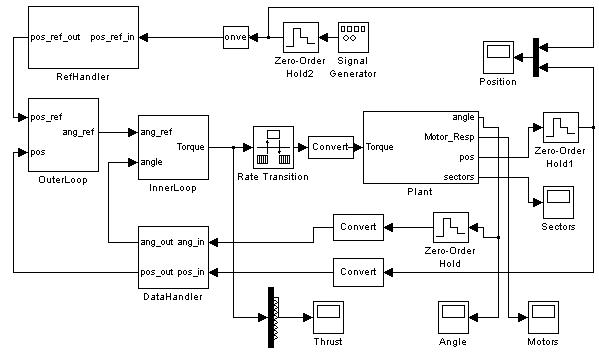
\includegraphics[width=\columnwidth]{figures/quad_integrator.jpg}
    \caption{High-level quad-integrator controller model}
    \label{fig:quad_integrator_model}
\end{figure}

The flight controller is divided into three primary subsystems:
DataHander, InnerLoop and OuterLoop.  The DataHandler block receives
the GPS and IMU sensor data and performs some simple unit conversions.
The InnerLoop controls the first two integrators in the
quad-integrator model which relate a saturated limited control-torque
$|\tau| \leq \tau_{\max}$ to the corresponding 
angular-velocity $\omega(t)=\dot{\theta}(t)$ and angular-position
$\theta$ of a rotational body with inertia $J$ such that
$J\dot{\omega}(t)=\tau(t)$ holds.  In order to control angular-position a
passive discrete-time proportional-derivative controller is
implemented periodically with a zero-order-hold (ZOH) at time $t=kT_s$ 
(in which $T_s$ is the sample-rate and $k$ is an integer) in the 
InnerLoop block such that $\tau(t) = k_p (\theta_d(k) - \theta(k)) - k_d 
\omega(k),\ t\ \in [kT_s,(k+1)T_s)$.  The resulting angular position
is equal to the control force applied to a body with mass $m$ such
that its velocity $v(t)=\dot{x}(t)$ and position $x$ are related such that
$\theta = m \dot{v}$.  Therefore, the OuterLoop control block 
determines the desired angular-position set-point $\theta_d$ to be
sent to the InnerLoop controller using a saturated passive
proportional-derivative controller such that
$\theta_{\mathsf{du}}(k)=k_{\mathsf{po}}(x_d(k)-x(k))
-k_{\mathsf{do}}v(k)$
\begin{equation*}
 \theta_d = \begin{cases}
\theta_{\mathsf{du}},\ \text{ if } |\theta_{\mathsf{du}}| \leq
\theta_{\max}\\
\mathsf{sgn}(\theta_{\mathsf{du}})\theta_{\max},\ \text{otherwise.}
\end{cases}
\end{equation*}
Finally, it is assumed that only $\theta$ and $x$ are periodically
sampled, therefore the respective angular velocity $\omega(k)$ and
velocity $v(k)$ are approximated using the following passive high-pass
filter with roll-off time-constant $\tau_f > 0$:
\begin{equation*}
y(k)-c y(k-1) = \frac{1-c}{T_s}(u(k)-u(k-1)),\ c=\exp(-\frac{T_s}{\tau_f})
\end{equation*}
in which $(u(k),y(k))$ correspond to either $(\theta(k),\omega(k))$ or
$(x(k),v(k))$ respectively.  All three of these subsystems are
incorporated into the final TrueTime model.  The continuous-time plant
and trajectory reference(RefHandler) are also necessary in the
TrueTime model, but reside outside of the  TrueTime blocks.

The remainder of this paper is organized as follows: Section 2 discusses the steps necessary to prepare the model for TrueTime generation.  Section 3 describes the process and results of generating the TrueTime model.  Section 4 covers related work and Section 5 concludes the paper.